\de{ĐỀ THI HỌC KỲ I NĂM HỌC 2022-2023}{THPT Trường Chinh - Đề số 2}


%%%%%%%%%%%%%%======Bài 1
\begin{bt}%[0T1B3-1][0T1B3-2]%[Dự án đề kiểm tra HKI NH22-23- Nguyễn Mộng Hùng]%[THPT-TRƯỜNG-CHINH-2]
	Cho hai tập hợp $A=\left[-3;\dfrac{5}{2}\right)$, $B=(-2;4]$. Tìm $A \cap B$, $A \setminus B$.
	\loigiai{
		Ta có\\ 
		$\bullet~A\cap B=\left(-2;\dfrac{5}{2}\right)$.\\
		$\bullet~A \setminus B=\left[-3;-2\right]$.
	}
\end{bt} 
%%%%%%%%%%%%%%======Bài 2
\begin{bt}%[0T2B2-3]%[Dự án đề kiểm tra HKI NH22-23- Nguyễn Mộng Hùng]%[THPT-TRƯỜNG-CHINH-2]
Giải hệ bất phương trình bậc nhất hai ẩn:
	$$\heva{&2x-y+4\geq 0\\& 2x-3y\leq 0.}$$
	\loigiai{
		$\bullet$ Đường thẳng $d_1\colon y=2x+4$ qua hai điểm $(0;4)$ và $(-2;0)$.\\
		$\bullet$ Đường thẳng $d_2\colon y=\dfrac{2}{3}x$ qua hai điểm $O(0;0)$ và $(3;2)$.
		\begin{center}
				\begin{tikzpicture}[line join=round, line cap=round,>=stealth,font=\footnotesize,scale=1]
					\begin{scope}
						\clip (-3.5,-3) rectangle (5,5);
						\fill[pattern=north west lines] (-3.5,-3)--(-3.5,5)--(0.5,5)--cycle;
						\fill[pattern=north west lines] (-6,-4)--(5,-3)--(6,4)--cycle;
						\draw (-3.5,-3)--(0.5,5) (0.5,4.5)node{$d_1$};
						\draw (-6,-4)--(6,4) (3.6,2.4)node [above] {$d_2$};
					\end{scope}
					\draw[->] (-3.5,0)--(5,0) node[below]{$x$};
					\draw[->] (0,-3)--(0,5) node[above]{$y$};
					\draw (0,0) node[above left]{$O$};			
					\draw(-2,0) node[below]{$-2$};
					\draw[fill=black]  (-2,0) circle (1.2pt);
					\draw(0,4) node[right]{$4$};
					\draw[fill=black]  (0,4) circle (1.2pt)(0,2) circle (1.2pt)(3,0) circle (1.2pt) (3,2) circle (1.2pt);
					\draw[dotted] (3,0)node[below]{$3$}--(3,2)--(0,2)node[left]{$2$};
				\end{tikzpicture}	
		\end{center}
	Miền nghiệm của hệ bất phương trình $\heva{&2x-y+4\geq 0\\& 2x-3y\leq 0}$ là phần không gạch sọc của hình trên.
}
\end{bt}
%%%%%%%%%%%%%%======Bài 3
\begin{bt}%[0T3B1-2]%[Dự án đề kiểm tra HKI NH22-23- Nguyễn Mộng Hùng]%[THPT-TRƯỜNG-CHINH-2]
	Tìm tập xác định của hàm số $y=\dfrac{2-\sqrt{3-x}}{x^2-4}+\dfrac{1}{\sqrt{x+4}}$.
	\loigiai{
		Hàm số xác định khi và chỉ khi
		$$\heva{&3-x\ge 0\\&x+4>0\\&x^2-4\neq 0}\Leftrightarrow\heva{&x\le 3\\&x>-4\\&x\neq\pm 2}\Leftrightarrow x\in(-4;3]\setminus\{-2;2\}.$$
		Vậy $\mathscr{D}=(-4;3]\setminus\{-2;2\}$.
	}
\end{bt}
%%%%%%%%%%%%%%======Bài 4
\begin{bt}%[0T3B2-1]%[Dự án đề kiểm tra HKI NH22-23- Nguyễn Mộng Hùng]%[THPT-TRƯỜNG-CHINH-2]
	Cho hàm số $y=-x^2-6x+7$.
	\begin{enumerate}
		\item Tìm tọa độ đỉnh, lập bảng biến thiên và chỉ ra các khoảng đơn điệu của hàm số trên.
		\item Hàm số đạt giá trị nhỏ nhất hay giá trị lớn nhất? Tìm giá trị đó.
	\end{enumerate}
	\loigiai{
		\begin{enumerate}
			\item $\bullet$ Gọi $S$ là tọa độ đỉnh của đồ thị hàm số trên, suy ra
			$$\heva{&x_S=\dfrac{-b}{2a}\\&y_S=\dfrac{-\Delta}{4a}}\Rightarrow\heva{&x_S=-3\\&y_S=16.}$$
			Vậy đỉnh của parabol là $S(-3;16)$.\\
			$\bullet$ Bảng biến thiên của hàm số $y=-x^2-6x+7$
			\begin{center}
				
\begin{tikzpicture}[>=stealth]
					\tkzTabInit[nocadre=false,lgt=1,espcl=2.5,deltacl=0.5]{$x$/.7,$y$/2}
					{$-\infty$ , $-3$ , $+\infty$}
					\tkzTabVar{-/$-\infty$ , +/$16$ , -/$-\infty$}
				\end{tikzpicture}
			\end{center}
		Dựa vào bảng biến thiên ta kết luận hàm số đồng biến trên khoảng $(-\infty;-3)$ và nghịch biến trên khoảng $(-3;+\infty)$.
		 \item Hàm số đạt giá trị lớn nhất trên $\mathbb{R}$ là $16$, không có giá trị nhỏ nhất trên $\mathbb{R}$.
		\end{enumerate}
	}
\end{bt}
%%%%%%%%%%%%%%======Bài 5
\begin{bt}%[0T6B4-1][0T6B4-2]%[Dự án đề kiểm tra HKI NH22-23- Nguyễn Mộng Hùng]%[THPT-TRƯỜNG-CHINH-2]
Cho biết điểm kiểm tra thường xuyên môn Lịch sử của $12$ học sinh như sau:\\[0.16cm]
\centerline{$7$; $7$; $9$; $8$; $10$; $10$; $5$; $8$; $9$; $9$; $7$; $10$}
\begin{enumerate}
	\item Tìm các tứ phân vị của mẫu.
	\item Viết công thức và tính phương sai của mẫu.
\end{enumerate}
	\loigiai{
		\begin{enumerate}
			\item Sắp xếp lại mẫu số liệu không giảm ta được\\
			\centerline{$5$; $7$; $7$; $7$; $8$; $8$; $9$; $9$; $9$; $10$; $10$; $10$}.\\
			$\bullet$ Vì cỡ mẫu $n=12$, là số chẵn nên giá trị tứ phân vị thứ hai là
			$$Q_2=\dfrac{1}{2}\cdot(8+9)=8{,}5.$$
			$\bullet$ Tứ phân vị thứ nhất là trung vị của mẫu $5;7;7;7;8;8$ Do đó
			$$Q_1=\dfrac{1}{2}\cdot(7+7)=7.$$
			$\bullet$ Tứ phân vị thứ ba là trung vị của mẫu $9;9;9;10;10;10$ Do đó
			$$Q_3=\dfrac{1}{2}\cdot(9+10)=9{,}5.$$
			\item Điểm trung bình môn Lịch sử của 12 học sinh là
			$$\overline{x}=(5+3\cdot7+2\cdot 8+3\cdot9+3\cdot 10):12=8{,}25.$$
			Phương sai của mẫu số liệu là
			\allowdisplaybreaks
			\begin{eqnarray*}
				S^2&=&\dfrac{1}{n}(x_1^2+x_2^2+x_3^2+\cdots+x_{12}^2)-\overline{x}^2\\
				   &=&\dfrac{1}{12}\cdot(7^2+7^2+9^2+8^2+10^2+10^2+5^2+8^2+9^2+9^2+7^2+10^2)-(8{,}25)^2\\
				   &=&2{,}1875.
			\end{eqnarray*}
		
		\end{enumerate}
}
\end{bt}



\begin{bt}%[0H4B3-1][Dự án đề kiểm tra HKI NH22-23- Tên Phạm Văn Long]%[THPT-TRƯỜNG-CHINH-2]
	Cho tam giác $ABC$ có $AB=4$, $BC=5$, $\widehat{B}=60^\circ$. Tính độ dài cạnh $AC$, diện tích tam giác $ABC$, bán kính đường tròn ngoại tiếp và bán kính đường tròn nội tiếp của tam giác $ABC$.
	\loigiai{
		Ta có 
		\begin{itemize}
			\item $AC=\sqrt{AB^2+BC^2-2\cdot AB\cdot BC\cdot \sin  B}=\sqrt{4^2+5^2-2\cdot 4\cdot 5\cdot \cos  60^\circ}=\sqrt{21}$.
			\item $S_{\triangle ABC}=\dfrac{1}{2}\cdot AB\cdot BC\sin B=\dfrac{1}{2}\cdot4\cdot 5\sin 60^\circ=5\sqrt{3}$.
			\item $\dfrac{AC}{\sin B}=2R\Rightarrow R=\dfrac{AC}{2\sin B}=\dfrac{\sqrt{21}}{2\sin 60^\circ}=\sqrt{7}$.
			\item $S=p\cdot r\Rightarrow r=\dfrac{S}{p}=\dfrac{5\sqrt{3}}{(4+5+\sqrt{21}):2}=\dfrac{3\sqrt{3}-\sqrt{7}}{2}$.
		\end{itemize}
		
	}
\end{bt}


\begin{bt}%[0H5K4-1][Dự án đề kiểm tra HKI NH22-23- Tên Phạm Văn Long]%[THPT-TRƯỜNG-CHINH-2]
Cho hình vuông $MNPQ$ tâm $O$ có cạnh bằng $3a$.
	\begin{enumerate}
		\item Dựng và tính độ dài véc-tơ $\vec{v}=\vec{MN}-\vec{PN}$.
		\item Gọi $K$ là trung điểm của $OP$. Phân tích $\vec{NK}$ theo hai vectơ $\vec{NM}$ và $\vec{NP}$.
		\item Tính tích vô hướng $\vec{MP} \cdot \vec{NM}$.
	\end{enumerate}
	\loigiai{
		\begin{center}
			\begin{tikzpicture}[>=stealth,smooth,line join=round,line cap=round,font=\footnotesize,scale=0.9]			
			\path
			(0,0) coordinate (M)
			(0,4) coordinate (N)
			(4,4) coordinate (P)
			(4,0) coordinate (Q)
			($(M)!0.5!(P)$) coordinate (O)
			($(O)!0.5!(P)$) coordinate (K);
			\draw (M)--(N)--(P)--(Q)--(M) (M)--(P) (N)--(Q) (N)--(K);
			\foreach \x/\g in {M/180,N/90,P/90,Q/05,O/0,K/-10} \fill[black] (\x) circle (1pt)+(\g:3.5mm) node{$\x$};
		\end{tikzpicture}
		\end{center}
	\begin{enumerate}
		\item Ta có $MNPQ$ là hình vuông nên $\vec{v}=\vec{MN}-\vec{PN}=\vec{MP}$.\\
		Do đó $\left|\vec{v}\right|=\left|\vec{MP}\right|=3a\sqrt{2}$.
		\item Ta có $\vec{NK}=\vec{NP}+\vec{PK}=\vec{NP}+\dfrac{1}{4}\vec{PM}=\vec{NP}+\dfrac{1}{4}\left(\vec{NM}-\vec{NP}\right)=\dfrac{1}{4}\vec{NM}+\dfrac{3}{4}\vec{NP}$.
		\item Ta có 
		\allowdisplaybreaks
		\begin{eqnarray*}
		\vec{MP} \cdot \vec{NM}&=&-\vec{MP} \cdot \vec{MN}\\
		&=&-\left|\vec{MP}\right| \cdot \left|\vec{MN}\right|\cdot \cos (\widehat{NMP})\\
		&=&-3a\sqrt{2}\cdot 3a\cdot \cos (45^\circ)=-9a^2.	
		\end{eqnarray*}
	\end{enumerate}
	}
\end{bt}

\begin{bt}%[0D2G2-2][Dự án đề kiểm tra HKI NH22-23- Tên Phạm Văn Long]%[THPT-TRƯỜNG-CHINH-2]
	\begin{enumerate}
		\item Tại một đài kiểm lâm, người ta phát hiện có một đám cháy. Cách đài kiểm lâm $50$ (m) có một bồn nước. Bằng máy trắc địa, người ta đo được góc nhìn từ bồn nước tới đài kiểm lâm và đám cháy là $97^\circ$; góc nhìn từ đài kiểm lâm tới bồn nước và đám cháy là $34^{\circ}$. Tính khoảng cách từ bồn nước tới đám cháy.
		\begin{center}	
			\tikzset{
				ex_markstyle/.style={},
				ex_mark/.style  n args={1}{decoration={ markings, %
						mark= at position 0.5 with
						with{
							\ifnum#1=1
							\draw[ex_markstyle] (0pt,-2pt) -- (0pt,2pt);
							\fi
							\ifnum#1=2
							\draw[ex_markstyle] (-1pt,-2pt) -- (-1pt,2pt);
							\draw[ex_markstyle] (1pt,-2pt) -- (1pt,2pt);
							\fi
							\ifnum#1=3
							\draw[ex_markstyle] (-2pt,-2pt) -- (-2pt,2pt);
							\draw[ex_markstyle] (0pt,-2pt) -- (0pt,2pt);
							\draw[ex_markstyle] (2pt,-2pt) -- (2pt,2pt);
							\fi
							\ifnum#1=4
							\draw[ex_markstyle] (-1pt,-1pt) -- (1pt,1pt);
							\draw[ex_markstyle] (-1pt,1pt) -- (1pt,-1pt);
							\fi
					} },
					pic actions/.append code=\tikzset{postaction=decorate}},
			}
			\definecolor{aureolin}{rgb}{0.99, 0.93, 0.0}
			\definecolor{amber}{rgb}{1.0, 0.75, 0.0}
			\definecolor{cadmiumorange}{rgb}{0.93, 0.53, 0.18}
			\definecolor{pastelbrown}{rgb}{0.51, 0.41, 0.33}
			\definecolor{skyblue}{rgb}{0.53, 0.81, 0.92}
			\definecolor{spirodiscoball}{rgb}{0.06, 0.75, 0.99}
			%---------------
			\definecolor{darkpastelblue}{rgb}{0.47, 0.62, 0.8}
			\definecolor{arylideyellow}{rgb}{0.91, 0.84, 0.42}
			\definecolor{cadet}{rgb}{0.33, 0.41, 0.47} %xám vỏ đèn
			\definecolor{phthalogreen}{rgb}{0.07, 0.21, 0.14} %màu giá đỡ đèn
			\definecolor{chocolate(traditional)}{rgb}{0.48, 0.25, 0.0} %hành lang
			\definecolor{persiangreen}{rgb}{0.0, 0.65, 0.58} %cửa kính
			\definecolor{pinegreen}{rgb}{0.0, 0.47, 0.44}
			\begin{tikzpicture}
				\clip (-12,-4) rectangle (3,6);
				\begin{pgfinterruptboundingbox}
					
					\tikzset{nha_gac/.pic={
							%----------------------------
							\def\D{ 
								(-1.1,.5)--(-1,-.9)--(1.05,-.9)--(1.108,.5)--cycle
								;}
							\draw[black] \D;
							\fill[persiangreen] \D;
							%----------------------------
							\def\C{ 
								(-.8,-.6)--(-.05,-.6)--(-.05,.2)--(-0.9,.2)--cycle
								(.8,-.6)--(.05,-.6)--(.05,.2)--(0.9,.2)--cycle
								;}
							\draw[black] \C;
							\fill[persiangreen!50] \C;
							%-----------------------------
							\def\K{ 
								(-.65,-.6)--(-.35,-.6)--(-.05,.2)--(-0.5,.2)--cycle
								(.3,-.6)--(.6,-.6)--(0.9,.2)--(.4,.2)--cycle
								;
								\fill[rectangle,red] (0,2.7)--(1,2.7)--(1,1.9)--(0,1.9)-- cycle;
								\draw[color=black!80!, line width=.3] (0,1.25)--(0,2.7);
								\node at (.5,2.3) (0,0)[star,fill=yellow,star point ratio=1.5,star point height=7.5pt,scale=.4] {};
							}
							\draw[black] \K;
							\fill[white] \K;
							%=================================
							\def\D{ %mái nhà
								(-1.9,.4)--(0,1.45)--(1.9,.4)--cycle
								;}
							%\draw[black] \D;
							\fill[red!80!black] \D;
							%------------------Chân trạm
							\draw[color=pinegreen!90, line width=1] (-.8,-4.2)--(-.8,-1.2)--(.8,-1.2)--(.8,-4.2)
							
							(-.8,-1.2)--(.8,-2.1) (-.8,-2.1)--(.8,-1.2)
							(-.8,-2.2)--(.8,-3.1) (-.8,-3.1)--(.8,-2.2);
							\fill[color=pinegreen] (-1.4,-.9)--(1.4,-.9)--(1.3,-1.15)--(-1.3,-1.15)--cycle;
					}}
					%%%%%%%%===========Tháp nước
					\tikzset{thap_nuoc/.pic={
							%------------------Chân trạm
							\def\D{ %bồn nước
								(-1,-.4)--(-1.3,0)--(-1.3,.4)--(-1,1)--(0,1.3)--(1,1)--(1.3,.4)--(1.3,0)--(1.1,-.4)--cycle
								;}
							\draw[color=spirodiscoball, line width=1] (-.9,-4.2)--(-.7,-.4)--(.7,-.4)--(.9,-4.2)
							(0,-.4)--(0,-4.2) (0,1.2)--(0,1.9)
							(-.8,-1.2)--(.8,-2.1) (-.8,-2.1)--(.8,-1.2)
							(-.8,-2.2)--(.8,-3.1) (-.8,-3.1)--(.8,-2.2);
							\draw[black] \D;
							\fill[skyblue] \D;
							;
					}}
					%%%%%%%%%%%==========ngọn lửa
					\tikzset{ngon_lua_3/.pic={
							\def\c{
								(0,-1.4)
								..controls +(170:.8) and +(-125:.5) ..(-.65,0)
								..controls +(55:1.2) and +(-85:.5) ..(-.1,1.4)
								..controls +(-40:.8) and +(85:.5) ..(.6,-.2)
								..controls +(40:.1) and +(-105:.15) ..(.75,.1)
								..controls +(-65:.5) and +(5:1) ..cycle
								;}
							\draw\c;
							\fill[cadmiumorange] \c;
					}}
					%------------------------
					
					\tikzset{ngon_lua_1/.pic={
							\def\c{
								(0,-1.4)
								..controls +(170:.8) and +(-125:.5) ..(-.65,0)
								..controls +(55:1.2) and +(-85:.5) ..(-.1,1.4)
								..controls +(-40:.8) and +(85:.5) ..(.6,-.2)
								..controls +(40:.1) and +(-105:.15) ..(.75,.1)
								..controls +(-65:.5) and +(5:1) ..cycle
								;}
							\draw\c;
							\fill[aureolin] \c;
					}}
					\tikzset{ngon_lua_2/.pic={
							\def\d{
								(0,-1.4)
								..controls +(170:.8) and +(-125:.5) ..(-.65,0)
								..controls +(55:1.2) and +(-85:.5) ..(-.1,1.4)
								..controls +(-40:.8) and +(85:.5) ..(.6,-.2)
								..controls +(40:.1) and +(-105:.15) ..(.75,.1)
								..controls +(-65:.5) and +(5:1) ..cycle
								;}
							\draw\d;
							\fill[amber!80] \d;
					}}
					%%%%%%%%%%%===============
					\node at (-5.7,2.5){\large $50$ m};
					\node at (-1,5){\large Bồn nước};
					\node at (-9,1.5){\large Đài kiểm lâm};
					
					\path 	(-9,-1.75) coordinate (A)
					(-3,4.75) coordinate (B)
					(0,0) coordinate (C)
					;
					\draw (B)--(C)--(A)--cycle;
					
					%---------------------------------------------------
					\path(-9,-1)pic[scale=.7]{nha_gac};
					\path(-3,5)pic[scale=.6]{thap_nuoc};
					\path
					(.7,-.6)pic[scale=.6,rotate=-35]{ngon_lua_3}
					(.5,0.2)pic[scale=.4,rotate=-25]{ngon_lua_3}
					(-.5,-.6)pic[scale=.6,rotate=210,yscale=-1]{ngon_lua_3}
					(-.4,.2)pic[scale=.4,rotate=180,yscale=-1]{ngon_lua_3}
					(0,0)pic[scale=1]{ngon_lua_2}
					(0,-.7)pic[scale=.5]{ngon_lua_1};
					
					\draw    pic["\large $34^\circ$", draw=black, angle eccentricity=1.4,angle radius=1.2cm, color=black]
					{angle=C--A--B};
					\draw    pic["\large $97^\circ$", draw=black, angle eccentricity=1.7, ex_mark=1,angle radius=.5cm, color=black]
					{angle=A--B--C};
					
					
				\end{pgfinterruptboundingbox}
			\end{tikzpicture}
		\end{center}
		\item \immini{Một người chạy bộ trong thời gian $2$ giờ với vận tốc $v$ (km/h) phụ thuộc thời gian $t$ (h) có đồ thị là một phần parabol với đỉnh $I(1;8)$ và trục đối xứng song song trục tung như hình bên. Tính vận tốc tức thời tại phút $90$ kể từ lúc bắt đầu chạy.
		\item  Một công ty, trong một tháng cần sản xuất ít nhất $12$ viên kim cương to và $9$ viên kim cương nhỏ. Từ $1$ tấn carbon loại I (giá $100$ triệu đồng) có thể chiết xuất được $6$ viên kim cương to và $3$ viên kim cương nhỏ. Từ $1$ tấn carbon loại II (giá $40$ triệu đồng) có thể chiết xuất được $2$ viên kim cương to và $2$ viên kim cương nhỏ. Mỗi viên kim cương to có giá $20$ triệu đồng, mỗi viên kim cương nhỏ có giá $10$ triệu đồng. Hỏi trong một tháng công ty này thu về được nhiều nhất là bao nhiêu tiền? Biết rằng mỗi tháng chỉ có thể sử dụng tối đa $4$ tấn carbon mỗi loại.}
		{	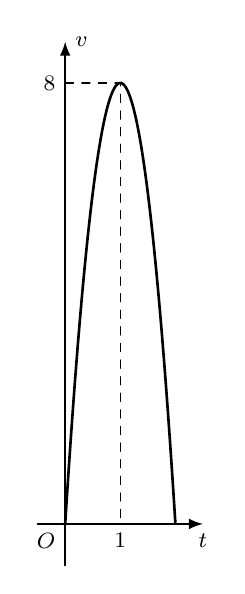
\begin{tikzpicture}[scale=0.7, font=\footnotesize,line join=round, line cap=round, >=stealth];
				\def\xt{-0.5} \def\xp{2.5} \def\yt{8.75} \def\yd{-0.75} % x_trái, x_phải, y_trên, y_dưới (giới hạn)
				%ve truc	
				\draw[-latex,line width=0.75pt] (\xt,0)--(\xp,0) node [below]{$t$};
				\draw[-latex,line width=0.75pt] (0,\yd)--(0,\yt) node [right]{$v$};
				\node at (0,0) [below left]{$O$};
				
				%ve do thi
				\clip (\xt-0.1,\yd+0.1) rectangle (\xp-0.1,\yt-0.1);
				\draw[line width=0.95pt,smooth,samples=300,domain=0:2] plot(\x,{-8*(\x)^2+16*(\x)}) ;
				\draw [dashed] (0,8)--(1,8)--(1,0) ;
				\draw (0,8) node [left] {$8$} ;
				\draw (1,0) node [below] {$1$} ;
				%ve doan thang								
			\end{tikzpicture}
		}
		
	\end{enumerate}
	\loigiai{
		\begin{enumerate}
			\item Đặt các điểm tại đài kiểm lâm, bồn nước, đám cháy lần lượt là các điểm $A, B, C$.\\
			Khi đó ta có $\widehat{A}=34^\circ, \widehat{B}=97^\circ\Rightarrow \widehat{C}=49^\circ$.\\
			Áp dụng định lý Sin vào $\triangle ABC$ ta có $$\dfrac{BC}{\sin A}=\dfrac{AB}{\sin C} \Rightarrow BC= \dfrac{AB\cdot \sin A}{\sin C}=\dfrac{50\cdot \sin 34^\circ}{\sin 49^\circ}\approx 37\,\mathrm{m}.$$ 
			\item Đặt $v(t)=at^2+bt+c$.\\
			Khi đó ta có hệ phương trình $\heva{&c=0\\&a+b+c=8\\&-\dfrac{b}{2a}=1}\Leftrightarrow \heva{&c=0\\&a+b+c=8\\&2a+b=0}\Leftrightarrow \heva{&a=-8\\&b=16\\&c=0.}$\\
			Suy ra $v(t)=-8t^2+16t$.\\
			Vận tốc tại $t=90'=1{,}5h$ là $v=-8\cdot (1{,}5)^2+16\cdot 1{,}5=6\, \mathrm{km/h}$.
			\item 
				Gọi $x, y$ lần lượt là số tấn Cacbon loại I và loại II  (với $x, y \geq 0$).\\
				Theo đề bài, ta có hệ bất phương trình $\heva{&6x+2y \geq 12 \\ &3x+2y \geq 9 \\ &0 \leq x \leq 4 \\ &0 \leq y \leq 4}$ \quad (I).\\
				Số tiền mua nguyên liệu là $100 x+40 y$ (triệu đồng).\\
				Số tiền bán là $20(6 x+2 y)+10(3 x+2 y)=150 x+60 y$ (triệu đồng).\\
				Lợi nhuận hàng tháng của công ty là $(150 x+60 y)-(100 x+40 y)=50 x+20 y$ (triệu đồng).\\
				Yêu cầu bài toán trở thành tìm $(x ; y)$ thỏa mãn (I) để $F(x ; y)=50 x+20 y$ đạt giá trị lớn nhất.\\
				Vẽ và xác định miền nghiệm của (I)\\
				Đặt $d_1\colon 6 x+2 y=12$, $d_2\colon 3 x+2 y=9$, $d_3\colon x=4$, $d_4\colon y=4$.
				\begin{center}
					\begin{tikzpicture}[scale=0.9, font=\footnotesize,line join=round, line cap=round, >=stealth];
						\fill[pattern=horizontal lines light gray,smooth] (-1,7)--(6,7)--(6,-1)--(-1,-1)--cycle;
						\fill[cyan,smooth] (2/3,4)--(4,4)--(4,0)--(3,0)--(1,3)--cycle;
						\draw[->] (-1,0) -- (6,0) node[below] {\scriptsize $x$};
						\draw[->] (0,-1) -- (0,7) node[left] {\scriptsize $y$};
						\draw (0.1,0.1)node[below left]{\scriptsize $O$};
						\draw[thin,samples=150,smooth,domain=-0.2:2.3] plot(\x,{-3*(\x)+6});
						\draw[thin,samples=150,smooth,domain=-1:3.5] plot(\x,{-1.5*(\x)+4.5});
						\draw (-1,4)--(6,4)	(4,-1)--(4,7);
						\draw (0.8,4)node[above]{$A$}  (4.2,4)node[above]{$B$} (4.2,0)node[above]{$C$} (2.5,0)node[above]{$D$} (0.8,3)node[below]{$E$};
						\draw  (4.2,0)node[below]{$4$} (2.8,0)node[below]{$3$} (1,0)node[below]{$1$} (0,3)node[left]{$3$};
						\draw[dashed] (1,0)--(1,3)-- (0,3);
						\draw[fill=black]  (2/3,4) circle (1.2pt) (4,4) circle (1.2pt)
						(4,0) circle (1.2pt) (3,0) circle (1.2pt) (1,3) circle (1.2pt);	
						\draw  (0,6)node[right]{$d_1$} (-0.2,5)node[left]{$d_2$} (4,6)node[right]{$d_3$} (6,4.2)node[left]{$d_4$};
					\end{tikzpicture}
				\end{center}
				Miền nghiệm của (I) là ngũ giác $ABCDE$ (kể cả biên).
				Khi đó ta có:
				\begin{itemize}
					\item $A\left(\dfrac{2}{3} ; 4\right), B(4 ; 4), C(4 ; 0), D(3 ; 0), E(1 ; 3)$ \\
					\item $F(x ; y)=50 x+20 y$. \\
					\item $F\left(\dfrac{2}{3} ; 4\right)=\dfrac{340}{3}$; $F(4 ; 4)=280$; $F(4 ; 0)=200$; $F(3 ; 0)=150$; $F(1 ; 3)=110$. \\				
				\end{itemize}
				Suy ra $\max F(x ; y)=F(4 ; 4)=280$.\\				
				Vậy trong một tháng công ty thu được nhiều nhất 280 triệu đồng tiền lãi.
		\end{enumerate}
	}
\end{bt}



